\chapter{Critical Systems}

\section{Critical Systems}


 If you are monitoring lots of hosts, getting an overview of which
 hosts need attention can be difficult. Most likely you've split the
 hosts among several pages, and the ``All non-green'' view is just
 cramped full with systems where a logfile is showing some errors, a
 filesystem needs cleaning up etc.



 The ``Critical Systems'' view lets you define exactly which tests on
 what hosts need attention. In other words, this is the view your
 Operations Center will be using to decide whether to call out people
 in the middle of the night. It might look like this:

\begin{figure} 
\centering 
\caption{critview-disk.png} 
\label{critview-disk.png} 
 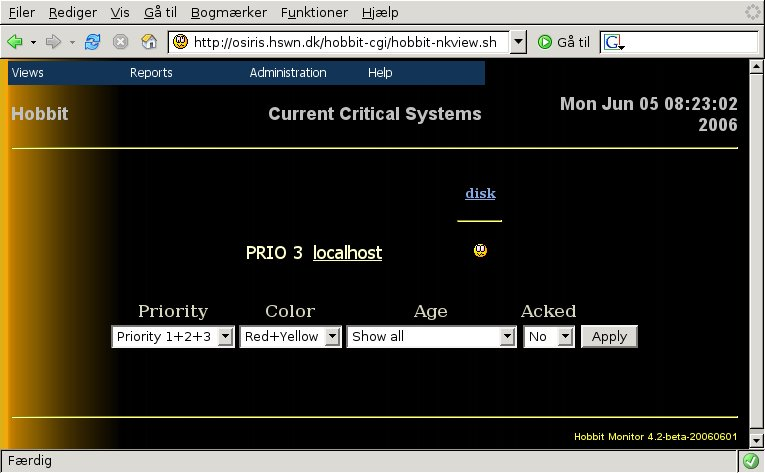
\includegraphics[scale=0.6]{./critview-disk.png} 
\end{figure}


 This document describes how you configure the Critical Systems view,
 and how it works for your operators. By ``operators'' I mean the
 people who are doing the 24x7 monitoring. Where I work, these people
 normally do not resolve the issues - they just raise the
 trouble-tickets and assign them to the ``engineer'' on duty. It may
 be different in your organization.

\section{The Critical Systems editor}


 To configure what goes on the Critical Systems view, you use a
 dedicated editor.



 The default Hobbit setup has nothing on the critical systems view. So
 to use it, you must configure some of your systems and tests to be
 included on this view. From the \textbf{Administration} menu, pick
 the \textbf{Edit Critical Systems} item. This is usually in the
 password-protected area of Hobbit, so you will need to authenticate
 yourself before you are allowed access. If you haven't set this up
 yet, look at the installation guide to see how you do that.



 After authenticating, you are presented with the editor page. 
\begin{figure}
\centering 
\caption{editor-main.png}
\label{editor-main.png}
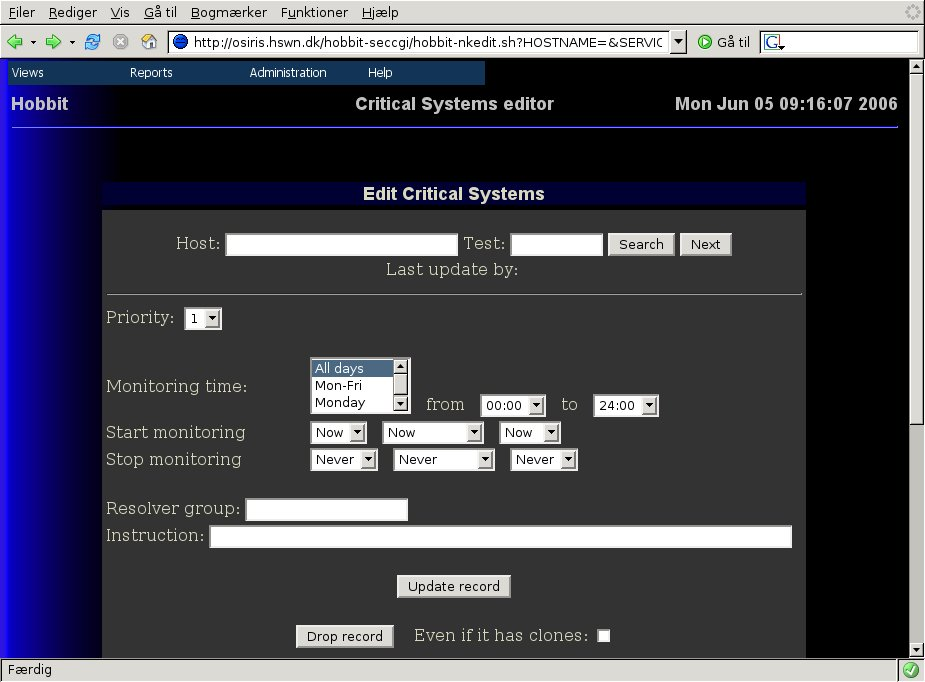
\includegraphics[scale=0.5]{./editor-main.png} 
\end{figure}

\subsubsection{The editor form} Let me explain what the various fields
are for: 

\begin{itemize}

\item The \textbf{Host}
 and \textbf{Test} fields are text entry fields. This is where you
 enter the name of the host and test you want to configure. If you
 would rather not type too much, you can enter just the beginning of
 the hostname and use the \textbf{Search} and \textbf{Next} buttons to
 walk through the currently configured tests.

\item The \textbf{Priority}
 field defines how important this test is. By default you have three
 priorities: 1, 2 and 3. Priority 3 is the lowest - things you must
 fix, but it can wait until you've had lunch or finished the
 department meeting. Priority 2 is for more important things, like one
 of your RAID systems running in degraded mode. Priority 1 is the
 highest priority - the kind of problem where you want to get a
 phonecall at 3 AM in the morning.

\item Then there is a group of time-related settings. The \textbf{Monitoring time}
 defines when this test should show up on the Critical Systems
 view. By default, that will be 24 hours a day, 7 days a week. But you
 probably have some systems that don't need attention during
 week-ends, or perhaps you only want to support a server during normal
 work-hours. Then you can use this setting to make sure it will only
 show up on the Critical Systems view during those periods. If you are
 migrating from the old ``NK'' settings in the bb-hosts file, this is
 the equivalent of the ``NKTIME'' setting. 

 The \textbf{Start monitoring} and \textbf{Stop monitoring} settings
 are used if you have systems that go into production at a certain
 date, or which are de-commisioned at a certain date. Instead of
 having to update your Critical Systems configuration exactly when
 that happens, you can configure the dates when monitoring of the
 systems should begin or end.

\item The \textbf{Resolver group}
 is a text field. You can use it for your operations people to see
 which group of engineers the should call about this problem. If you
 have multiple groups handling different parts of your IT systems, use
 this to let the operations staff know whether to call the Unix
 admins, the DBA's or one of your Webmasters.

\item The \textbf{Instruction}
 is a text entry field, where you can place a brief instruction to the
 operators handling the problem: If there is a simple thing that the
 operations people can try to fix the problem before calling the
 on-duty engineer, then you can place instructions here - e.g. perhaps
 the issue is with an external partner, so they just need to call them
 and let them know there is an issue. You can use HTML tags in this
 field, so if it's a long story then just put in an HTML link to
 another document.

\item The \textbf{Clone}
 fields at the bottom of the form (not visible in the screenshot) are described later

\end{itemize}
\subsubsection{Setting up a disk status}


 Right now, there is a yellow disk status on my system. 
\begin{figure} \centering \caption{test}\label{fig1}
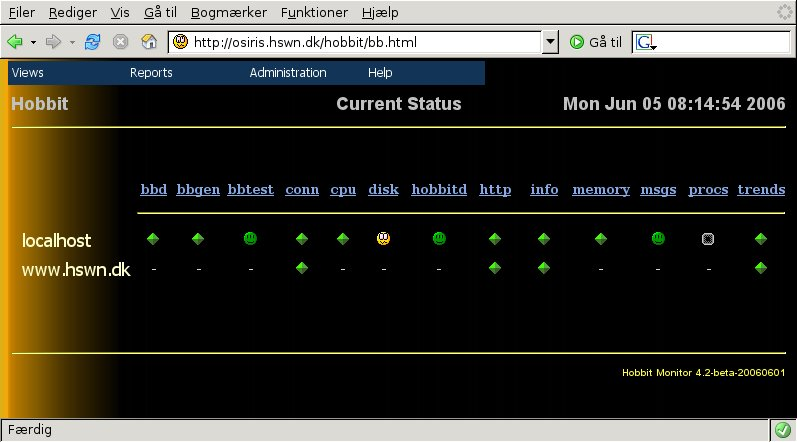
\includegraphics[scale=0.5]{./mainview.png} 
\end{figure}

 But it is not on the Critical Systems view, and I want it to be. It
 is a priority 3 event, and I only want it monitored between 7AM and
 8PM on weekdays. Most likely it is just some logfiles that are
 filling up, so the operators can try and clean out the /var/log/
 directory - if that doesn't solve the problem, then they must
 escalate it to the Unix admins.



 So on the Critical Systems editor, I enter the hostname \textbf{localhost}
 and the test \textbf{disk}
, then hit the \textbf{Search}
 button. I get this warning: 

\begin{figure} 
\centering 
\caption{editor-nohost.png}
\label{editor-nohost.png}
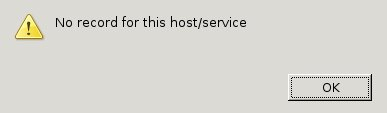
\includegraphics[scale=0.5]{./editor-nohost.png} 
\end{figure}

 telling me that there is nothing configured yet for this host+test
 combination. If there had been any previous configuration, it would
 have shown up on the form.



 So I fill out the fields of the form and hit the \textbf{Update}
 button. The form changes to look like this: 

\begin{figure}
\centering 
\caption{editor-diskchanged.png}
\label{editor-diskchanged.png}
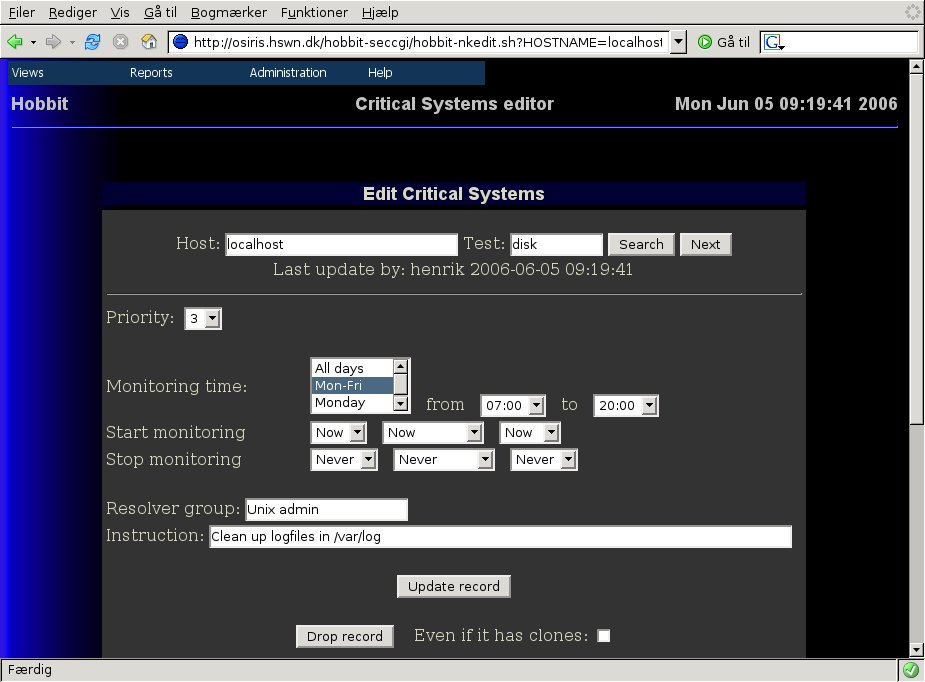
\includegraphics[scale=0.5]{./editor-diskchanged.png}
\end{figure}

 As you can see, there is now a \textbf{Last update}
 text showing who has changed this configuration, and when it was last done.


 If I now go back to the Critical Systems view - from the menu, pick \textbf{Views}
 and \textbf{Critical Systems view}
 - you will see that the status is now showing up: 

\begin{figure} \centering \caption{critview-disk.png}\label{critview-disk.png}
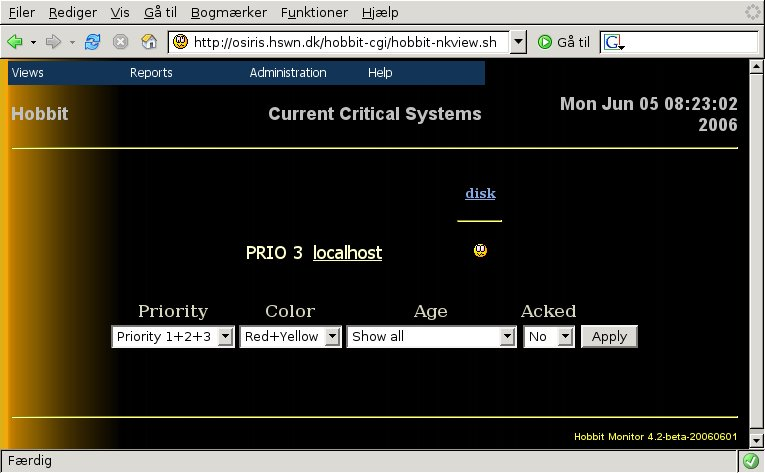
\includegraphics[scale=0.5]{./critview-disk.png} 
\end{figure}
\subsubsection{Template definitions - cloning records}


 If you have many hosts that share a common setup on the Critical
 Systems view, then editing all of them can be tiresome. Instead, you
 should define a template and then \textbf{clone} it to all of the
 hosts.



 NOTE: A cloned definition is not a copy of the original
 definition. It is in fact a pointer back to the original definition,
 so if you change the original definition \emph{after} you performed
 the cloning, then the clone definition will \emph{also} change.



 Defining a template is just like defining the Critical Systems view
 for a host. Just call the host something that looks like a template -
 ``\textbf{Standard Unix}``, for instance. So here is a definition for
 a \textbf{Unix cpu}  template. 

\begin{figure} \centering \caption{editor-clonemaster.png}\label{editor-clonemaster.png}
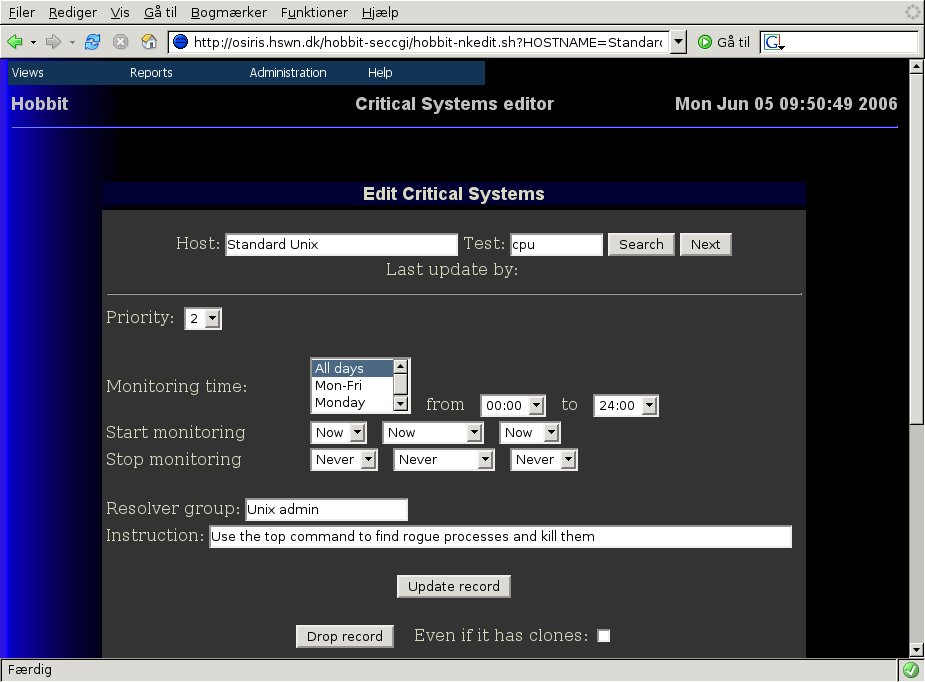
\includegraphics[scale=0.5]{./editor-clonemaster.png} 
\end{figure}

 Now we have created the template (if you haven't pushed the
 \textbf{Update}

 button to save the template, do it now). To apply this template to a
 host, scroll down to the bottom of the editor form, and enter the
 hostname that you want to apply the template to, then hit the
 \textbf{Add/remove clones} button: 

\begin{figure} \centering \caption{editor-makeclone.png}\label{editor-makeclone.png}
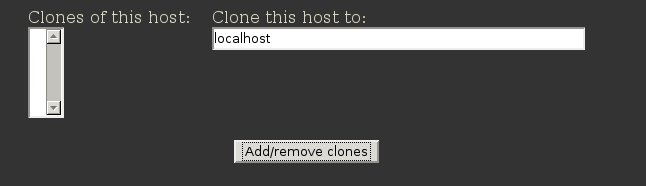
\includegraphics[scale=0.5]{./editor-makeclone.png} 
\end{figure}

 After it has updated, you can see that ``localhost'' is now listed in
 the scrollbox showing the clones. 

\begin{figure} \centering \caption{editor-showclone.png}\label{editor-showclone.png}
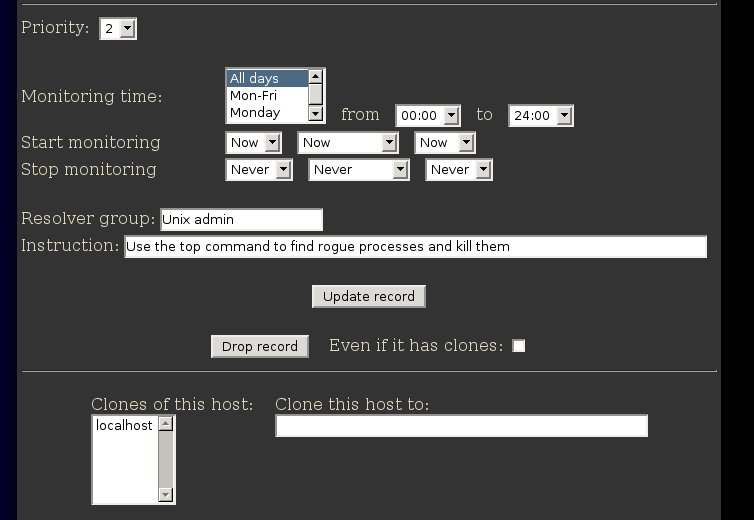
\includegraphics[scale=0.5]{./editor-showclone.png} 
\end{figure}

 NOTE: Cloning happens at the \textbf{host} level, so even though we
 did the cloning from a \textbf{cpu} test definition, it will also
 affect all the other definitions we have for the \textbf{Standard
 Unix} host.

\section{The Critical Systems view}


 The critical systems view lets the operators filter active alerts in
 several ways. It might look like this: 

\begin{figure} \centering \caption{critview-disk.png}\label{critview-disk.png}
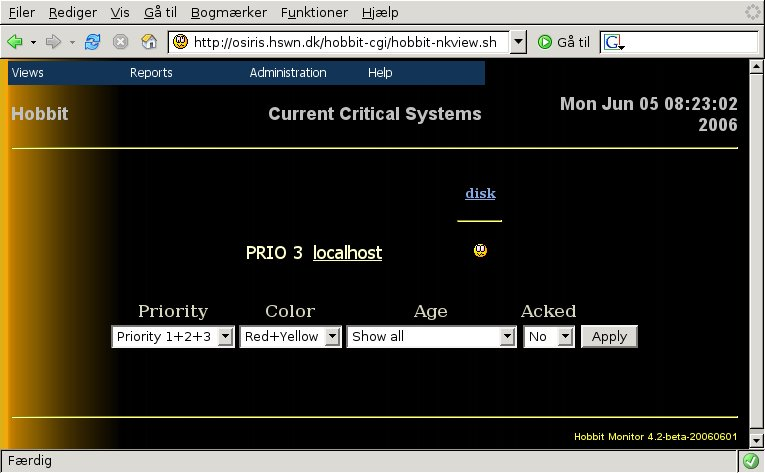
\includegraphics[scale=0.5]{./critview-disk.png} 
\end{figure}

\subsubsection{Filtering the Critical Systems view}


 The drop-down boxes lets the operators filter the alerts that show up
 on the page. 

\begin{itemize}
\item The \textbf{Priority}
 limits alerts so that only those with a matching priority get displayed.
\item The \textbf{Color}
 removes those alerts that have an unwanted color
\item The \textbf{Age}
 limit can be used to only see the most recent events.
\item The \textbf{Acked}
 selection can be used to toggle the view of events that have been acknowledged by the operators. 

\end{itemize}



 \textbf{Tip:}
 If you have a preferred default setting for these, then you can
 bookmark it in your browser - the settings are part of the URL, so
 your bookmark will include the current settings.

\subsubsection{The detailed status view}


 When looking at the status of one of the items shown on the Critical
 Systems view, a number of additional items show up. On the example
 Critical Systems view above, you will notice that the instructions we
 entered about what to do with the disk status is shown here, so they
 are available to the operators. There are links to the host
 documentation and host information. There is also an acknowledge
 function, so that the operators can acknowledge an alert right away.

\subsubsection{Critical Systems acknowledgment}


 From the detailed status view, the operator can \textbf{acknowledge}
 an alert, after he has assigned the problem to an engineer or has
 handled it in some other way. This serves two purposes: First, it
 removes the status from the Critical Systems view, so the operator
 can concentrate on the new problems that appear. And second, it lets
 everyone else see that the problem has been noticed and is being
 handled by someone.



 When acknowledging an alert, the operator can add information about
 what the problem is, or who is handling it, and when it is expected
 to be resolved. E.g. like this: 

\begin{figure} \centering \caption{critview-detail-ackform.png}\label{critview-detail-ackform.png}
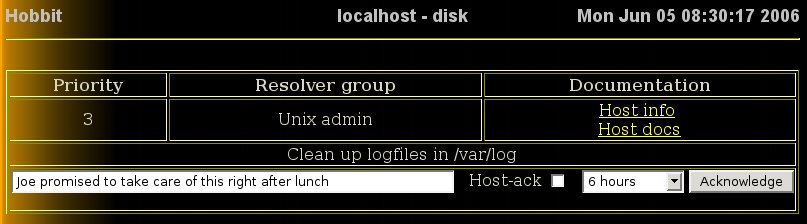
\includegraphics[scale=0.5]{./critview-detail-ackform.png} 
\end{figure}

 The \textbf{Host-ack} checkbox lets the operator acknowledge all
 current alerts for a given host, e.g. a full disk could easily
 trigger alerts for both the disk-, msgs- and procs-statuses - a Host
 ack lets him handle all of those.



 After the operator has acknowledged the status, the acknowledgment
 will be visible on the Critical systems status view: 

\begin{figure} \centering \caption{critview-detail-acked.png}\label{critview-detail-acked.png}
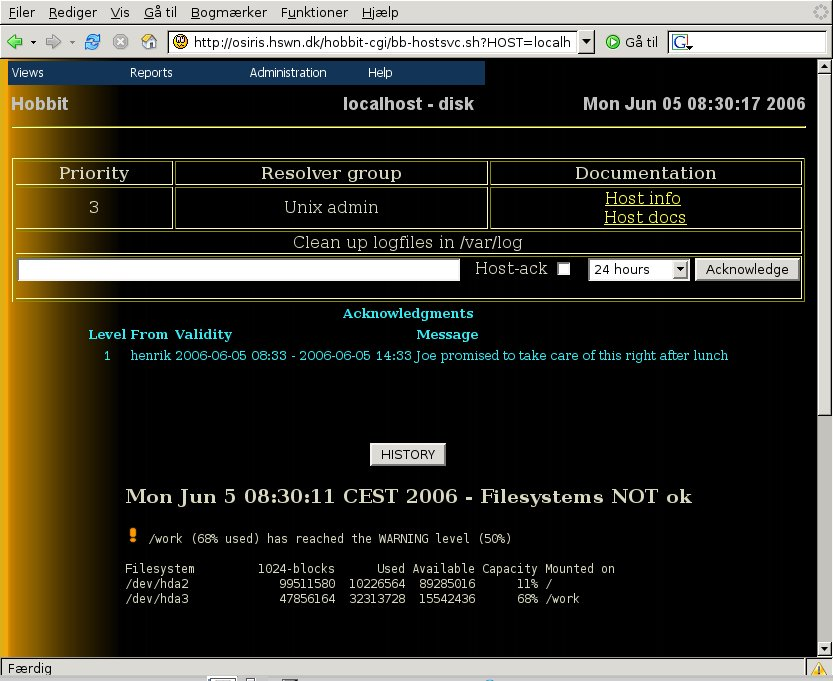
\includegraphics[scale=0.5]{./critview-detail-acked.png} 
\end{figure}

 (If you are wondering why this image says it is a ``Level 1''
 acknowledgement, then the answer is that a future release of Hobbit
 will allow multiple acknowledgments by different groups. Level 1 is
 the operator who sees the alert on the Critical Systems view. Level 2
 could be the engineer who gets paged by a Hobbit alert going
 out).

\subsubsection{How acknowledgements are visible to everyone}


 The acknowledgments that the operator enters from the status page
 will show up on the status visible to everyone. E.g. here is how the
 overview page will appear to a normal user: Note that the ``disk''
 status has a yellow checkmark, indicating that it has been
 acknowledged: 

\begin{figure} \centering \caption{mainview-acked.png}\label{mainview-acked.png}
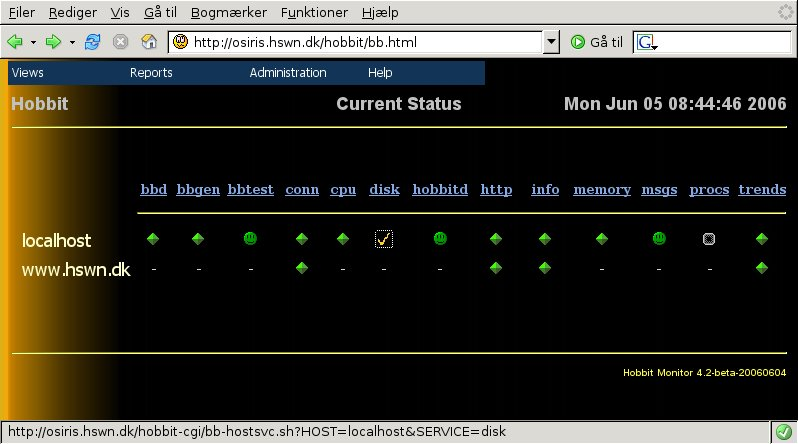
\includegraphics[scale=0.5]{./mainview-acked.png} 
\end{figure}

 And the detailed status page also includes the acknowledgment
 information: 

\begin{figure} 
\centering \caption{stdview-detail-acked.png}
\label{stdview-detail-acked.png}
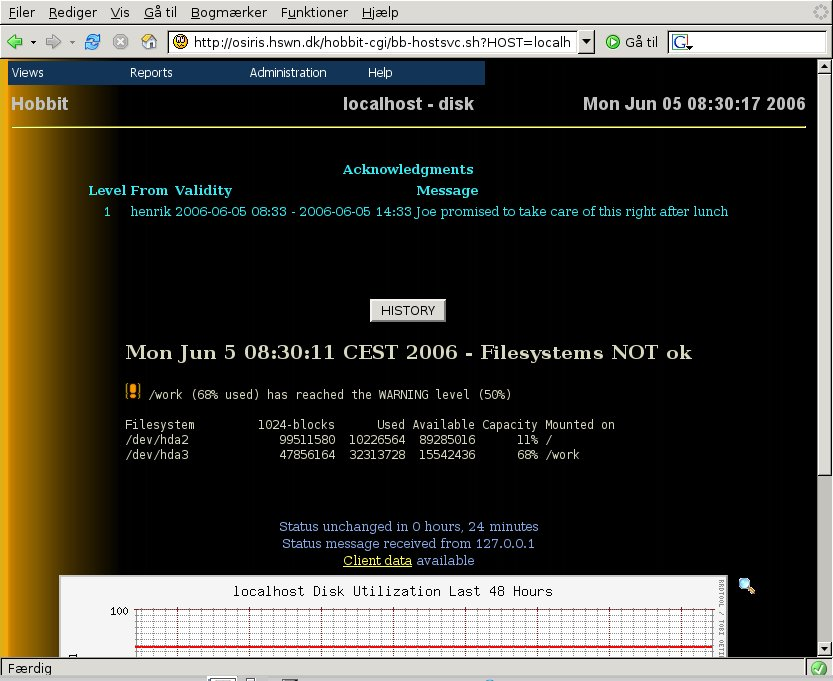
\includegraphics[scale=0.5]{./stdview-detail-acked.png} 
\end{figure}

